\section{Teilversuch 4: Babinetsches Theorem}
 	\subsection{Spalt/Streifen}
 		Das Beugungsmuster vom Spalt ist viel schöner als das vom Strich. Es gab viel Rauschen und für jedem Peak im Beugungsmuster des Spaltes gibt es viele kleine Peaks im Beugungsmuster des Striches. Grob kann man aber erkennen, dass die Peak-Intensitäten der beiden Beugungsmustern vielleicht an dem gleichen Positionen liegen (was unsere Theorie besagt). Der Abstand zwischen jeder dieser einhüllenden Maximalen bleibt aber ungefähr gleich.

 		Im Experiment war aber eine Verschiebung in dem Beugungsmuster zu erkennen. Ob das an einem experimentellen Fehler (zum Beipiel beim Umdrehen des Glasplättchens) oder an einer physikalisch grundliegende Ursache liegt, weiß ich leider nicht. Im Nachhinein sollte ich das ungeschobene Beugungsmuster des Striches auch ausgedrucken lassen, aber leider habe ich das Kamera schon geschoben.

 	\subsection{Loch/Punkt}
 		\begin{figure}[H]
		\centering
 			\begin{tabular}{c p{1em} c}
 				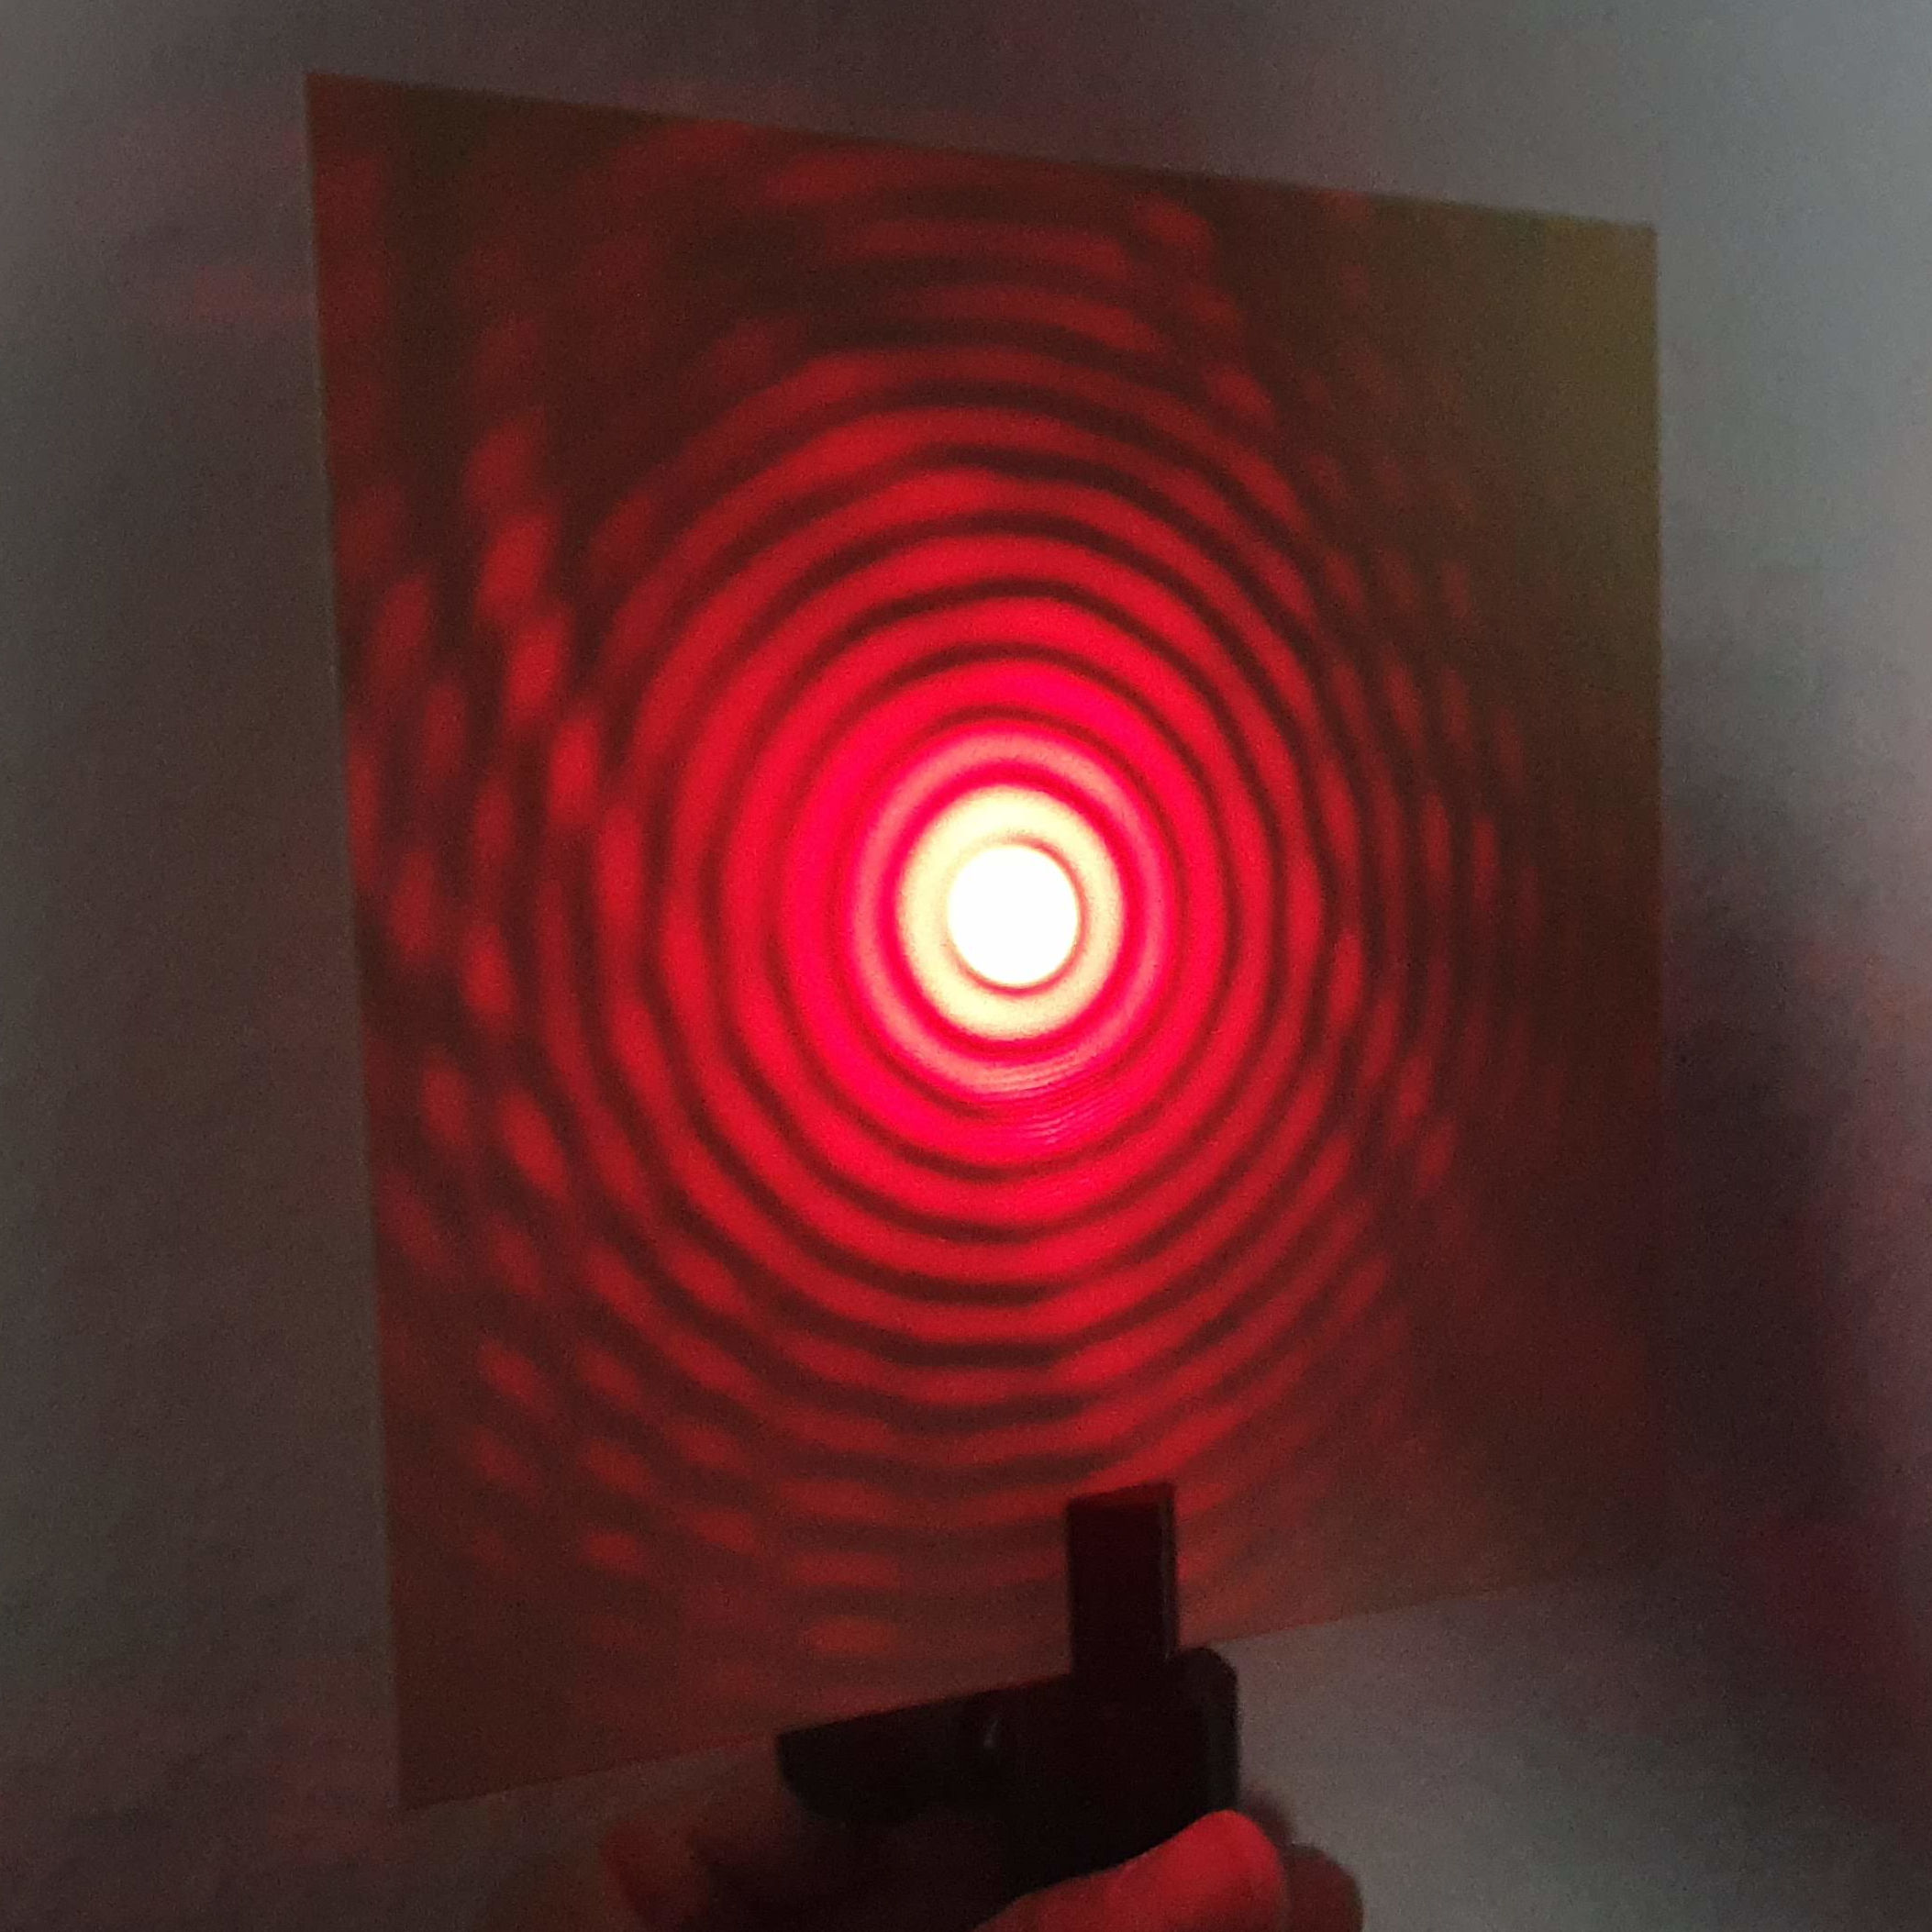
\includegraphics[width=0.4\textwidth]{images/tv4-hole.jpg} &&
 				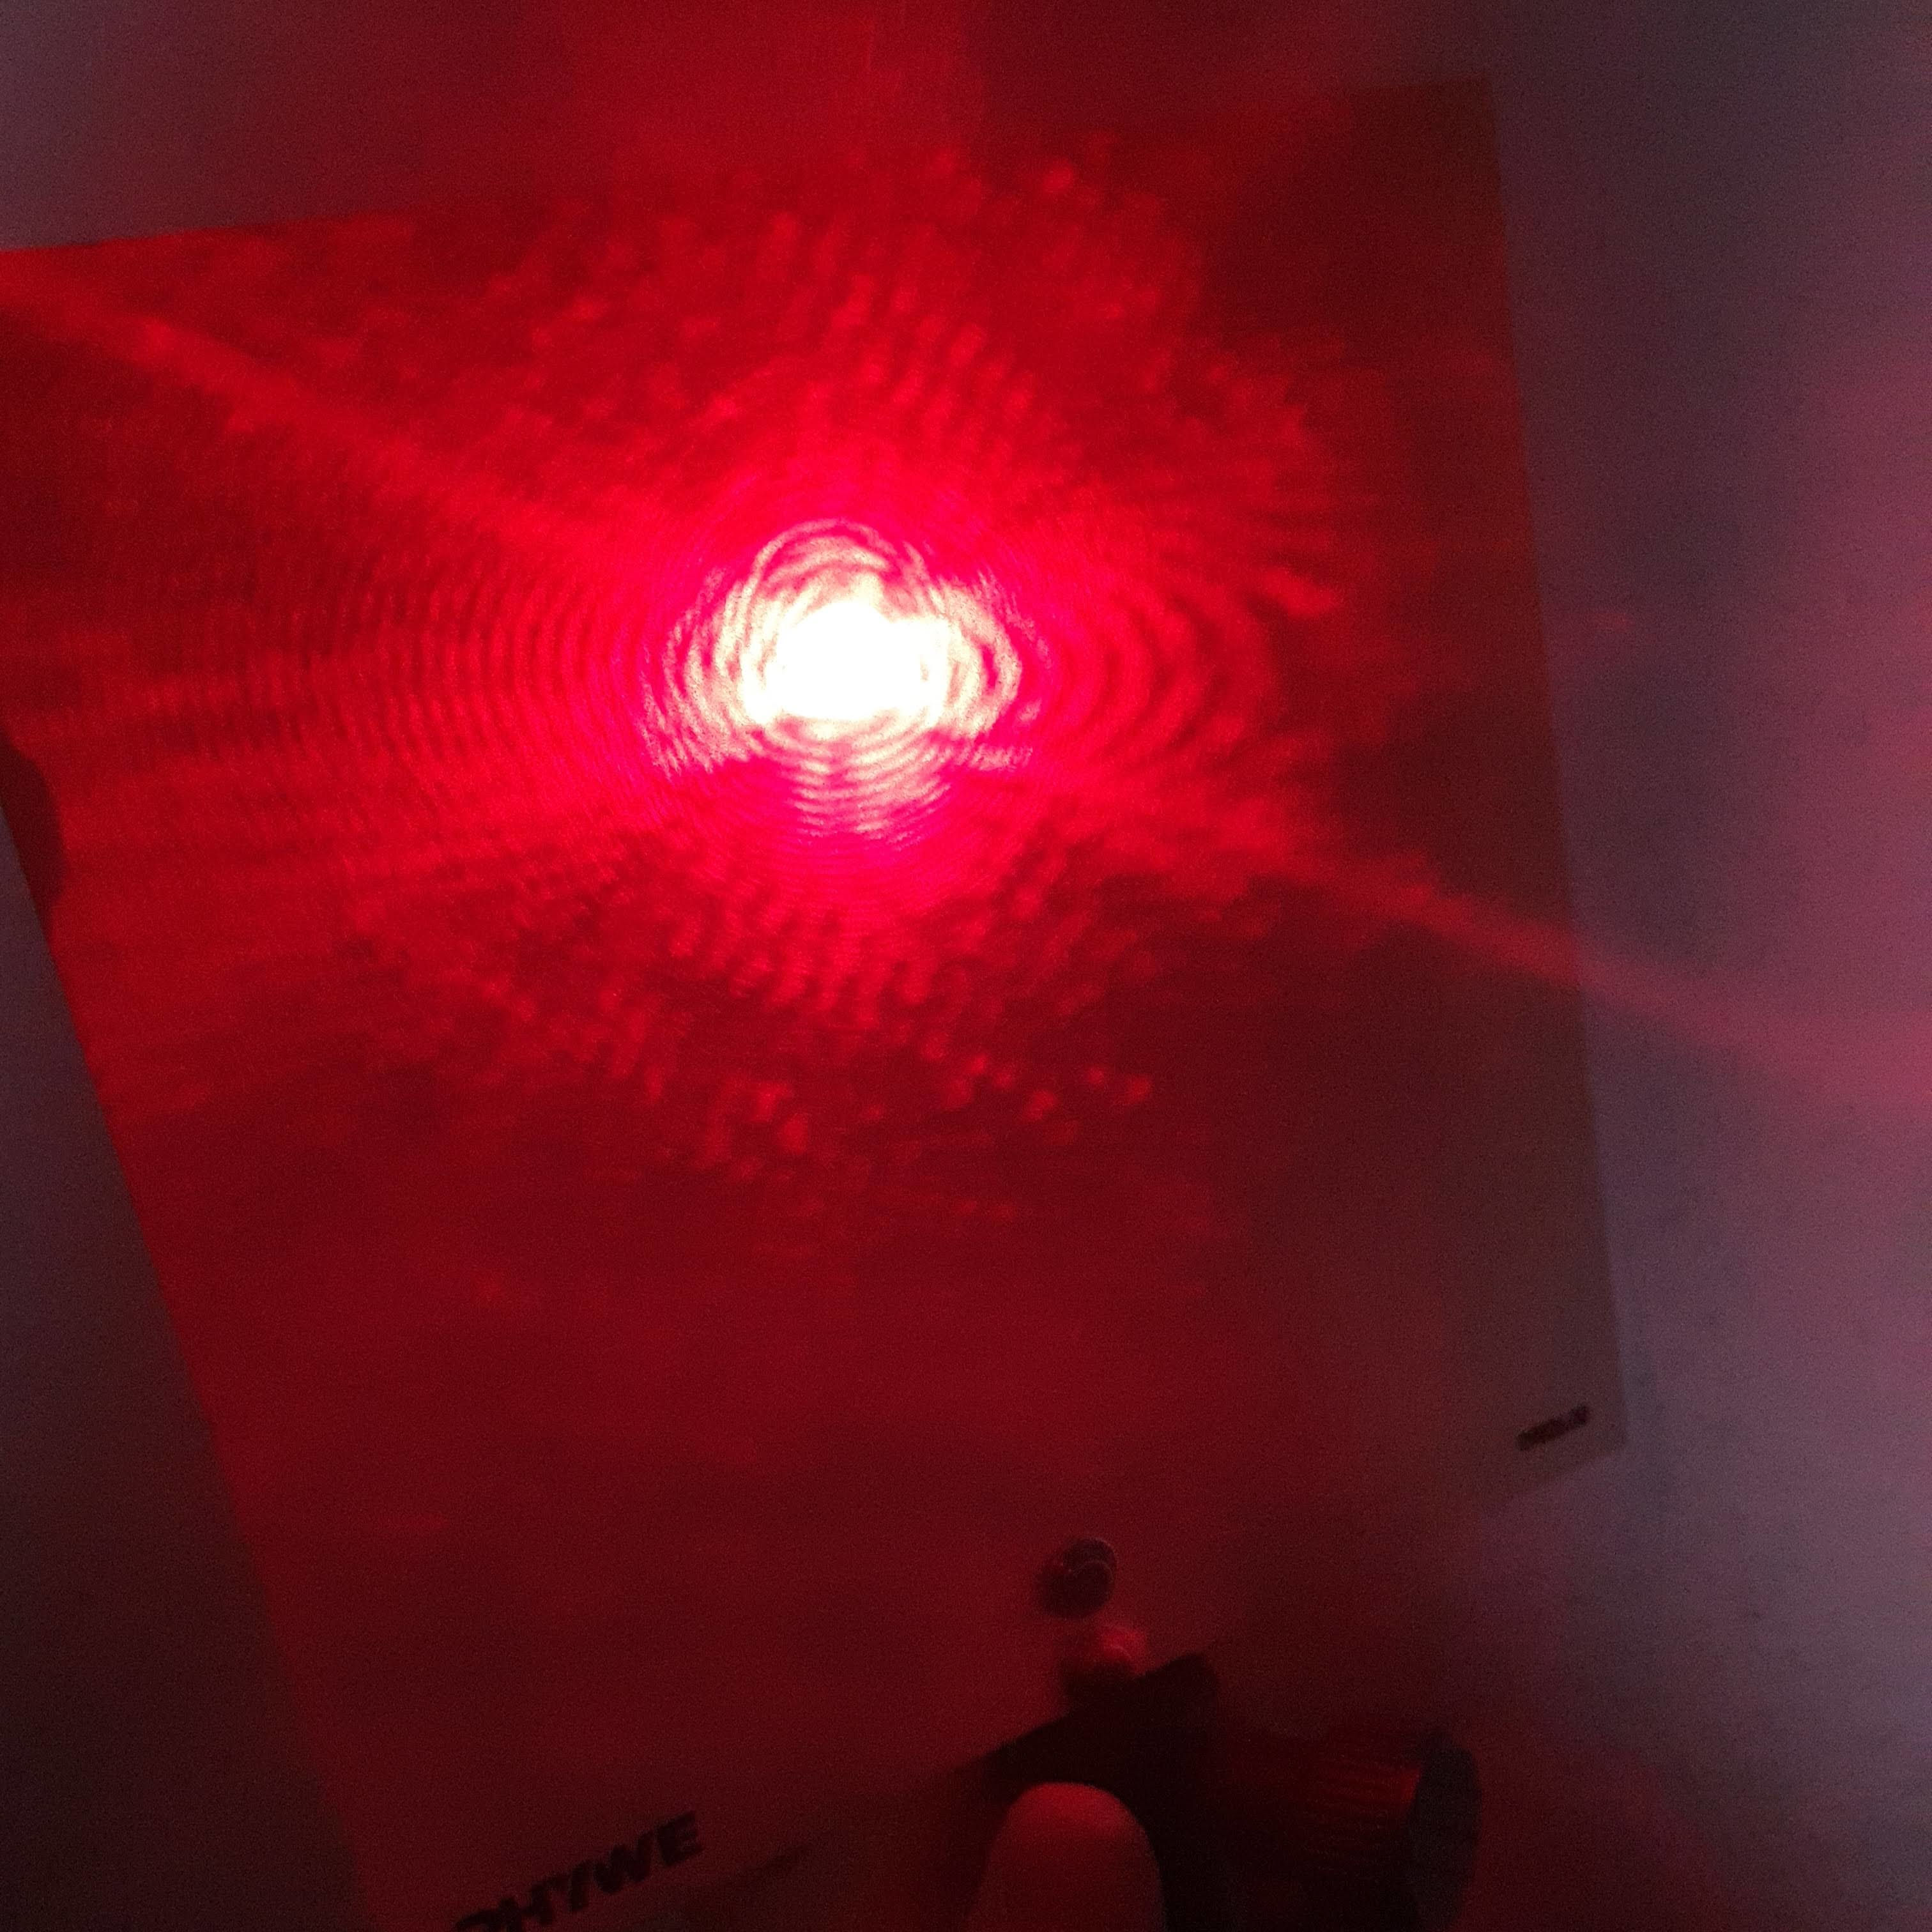
\includegraphics[width=0.4\textwidth]{images/tv4-dot.jpg} 
 			\end{tabular}
	 		\caption{\centering Beugungsmuster vom Loch (links) und Punkt (rechts)}
			\vspace{-1em}
		\end{figure}
		Das Beugungsmuster mit dem Loch hat einen höheren Kontrast im Vergleich zu dem mit dem Punkt. Dies könnte daran liegen, dass der Punkt nicht genau mittig im Laserstrahl stand. Es gibt aber im beiden Fällen etwa konzentrische kreisförmige Interferenzstreifen. Laut dem Babinetsches Theorem sollen komplementäre Blende das gleiche Interferenzmuster erzeugen. Da der Punkt und das Loch komplementäre zueinander sind, entspricht unsere Beobachtung unsere Erwartungen. 

		Im Fall des Punkts ist das Beugungsmuster sehr verzehrt und unsymmetrisch. Das Grund weiß ich nicht genau, aber vermütlich liegt es an dem Glasplättchen, das nicht senkrecht zum Laserstrahl lag. 

		Im Allgemein aber: je ferner man ist vom Zentrum, desto dunkler unseres Intereferenzmuster ist. Dies liegt daran, dass der Strahl Gaussförmig ist und die Intensität nimmt mit zunehmender Radius vom Zentrum. 

		Man erkennt außerdem (besonders im Fall des Lochs), dass es anscheinend ein einhüllenede Beugungsmuster außenrum gibt. Das könnte ein Artefakt des ursprunglichen Laserstrahl sein. Genau kann ich leider nicht erklären. 